\documentclass{beamer}
\setbeamertemplate{headline}[frame number]
\setbeamertemplate{section in toc}[sections numbered]
\setbeamertemplate{subsection in toc}[subsections numbered] 
\usetheme[left, hideallsubsections]{Goettingen} 
\usepackage[utf8]{inputenc}
\usepackage{amsmath}
\usepackage{subfigure}
 
 
\title{Group 6\\
	Pond Environmental Measurement\\
	SSNS - Smart Sensor Network Systems}
\author{Alexander K.,
	Sabrina B.,
	Rozana A.,
	Alexander V.D.}
 
\institute[FHF] {Fachhochschule Frankfurt am Main - University of Applied Sciences}

\date 
{\today}

\begin{document}

\maketitle
\begin{frame}
\frametitle{Table of Contents}
\tableofcontents
\end{frame}

%%%%%%%%%%%%%%%%%%%%%%%%%%%%%%% Project Describtion %%%%%%%%%%%%%%%%%%%%%%%%%%%%%%%%%%
\section{Project Describtion} 
\subsection{Idea}
\frame
{
	\frametitle{Project}
	\begin{figure}[h!]
  		\centering
    	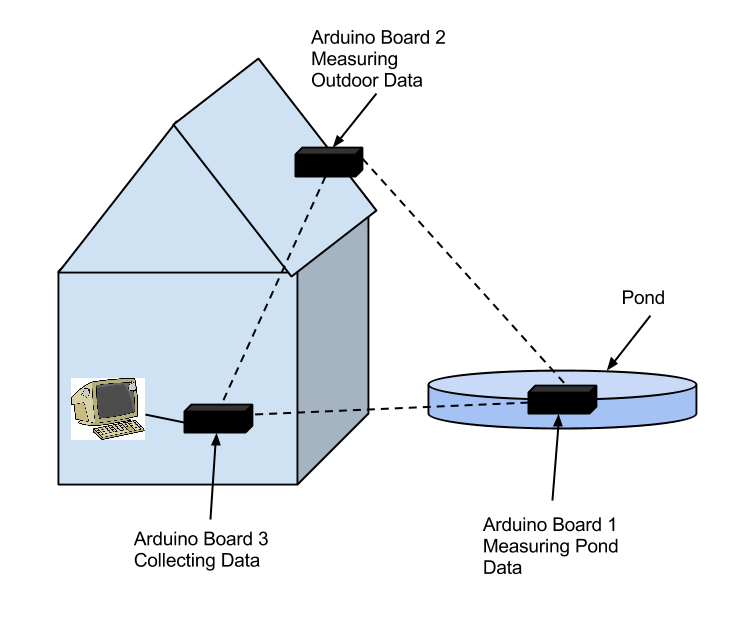
\includegraphics[width=0.85\textwidth]{../Images/ssns_project.png}
		\caption{Model}
	\end{figure}
}

\subsection{Requirements}
\frame
{
	\frametitle{System Requirements}
	\begin{itemize}
	\item reliable 24/7 data Aquisition
	\item Data being storaged on the collecting Node
	\item Graphical visualization on the PC
	\end{itemize}
}

\subsection{Project Plan}
\frame
{
	\frametitle{}
	\begin{center}
	Project Plan	
	\end{center}
}

%%%%%%%%%%%%%%%%%%%%%%%%%%%%%% Hardware %%%%%%%%%%%%%%%%%%%%%%%%%%%%%%%%%%%%%%%%%%%%%%%%
\section{Hardware}
\frame
{
	\frametitle{Hardware}
	Hardware
	\begin{itemize}
	\item Ardiuno UNO module
 	\item Arduino Wireless SD
	\item XBee ProSeries 2XBP24-Z7 module
	\item The Sensors
	\end{itemize}
	IDE installation	
}

\frame
{
	\frametitle{Arduino UNO module}
	\begin{figure}[h!]
  		\centering
    	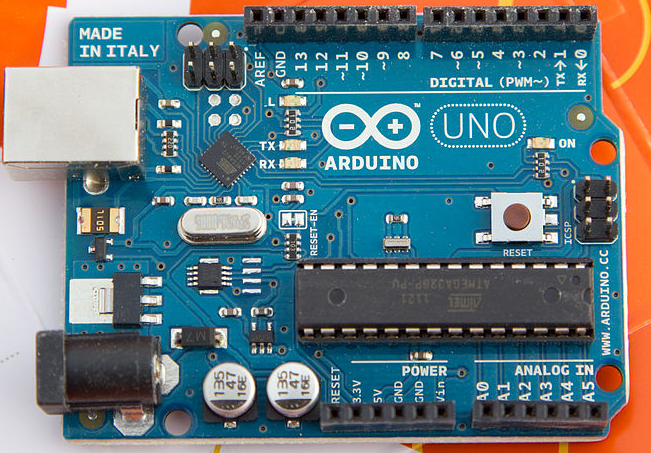
\includegraphics[width=0.85\textwidth]{../Images/Arduino_Uno.png}
		\caption{Arduino Uno}
	\end{figure}
}

\frame
{
	\frametitle{Arduino UNO module}
	\begin{itemize}
	\item An Arduino board consists of an Atmel 8-bit AVR microcontroller with complementary components to facilitate programming and incorporation into other circuits.
	\item An important aspect of the Arduino is the standard way that connectors are exposed, allowing the CPU board to be connected to a variety of interchangeable add-on modules known as shields. 
	\end{itemize}
}

\frame
{
	\frametitle{Wireless SD Shield}
	\begin{figure}[h!]
  		\centering
    	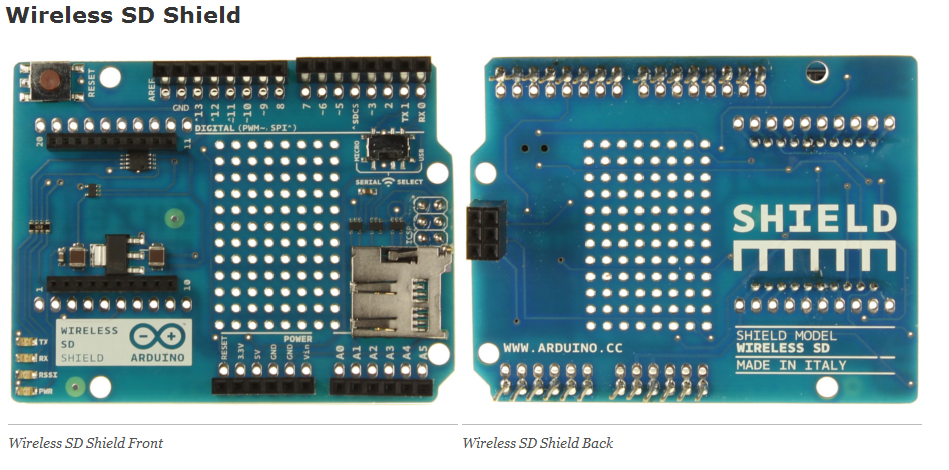
\includegraphics[width=\textwidth]{../Images/Arduino_WS.png}
		\caption{Arduino Wireless SD Shield}
	\end{figure}
}

\frame
{
	\frametitle{Wireless SD Shield}
	\begin{itemize}
	\item The Wireless SD shield allows an Arduino board to communicate wirelessly using a wireless module.
 	\item It is based on the Xbee modules from Digi, but can use any module with the same footprint.
 	\item The module can communicate up to 100 feet indoors or 300 feet outdoors (with line-of-sight).
 	\item It can be used as a serial/usb replacement or you can put it into a command mode and configure it for a variety of broadcast and mesh networking options. 
	\item The shields breaks out each of the Xbee's pins to a through-hole solder pad. 
	\end{itemize}
}

\frame
{
	\frametitle{XBee ProSeries 2XBP24-Z7 module}
	\begin{figure}	
	\subfigure[Xbee Module front]{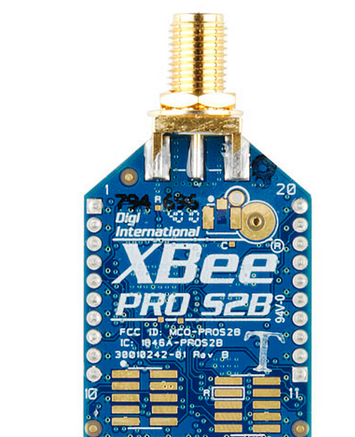
\includegraphics[width=0.49\textwidth]{../Images/Xbee_1.png}}
	\subfigure[Xbee Module back]{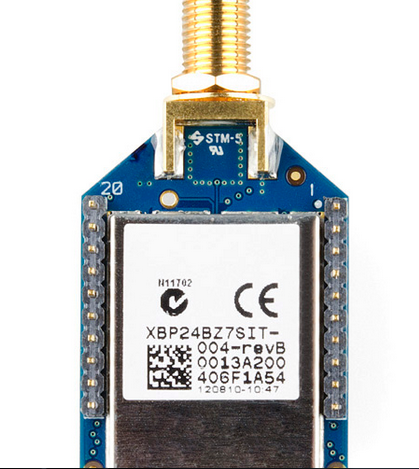
\includegraphics[width=0.49\textwidth]{../Images/Xbee_2.png}}
	\end{figure}	
}

\frame
{
	\frametitle{XBee ProSeries 2XBP24-Z7 module}
	\begin{enumerate}
	\item Allow to complex mesh networks based on the XBee ZB ZigBee mesh firmware. 
	\item These modules allow a very reliable and simple communication between microcontrollers, computers, systems, really anything with a serial port! 
	\item Point to point and multi-point networks are supported.
	\end{enumerate}		
}

\frame
{
	\frametitle{Integrated developement environment}
	The Arduino IDE is a cross-platform application written in Java, and is derived from the IDE for the Processing programming language and the Wiring projects. 
}

\frame
{
	\frametitle{Integrated developement environment}
	It includes a code editor with features such as syntax highlighting, brace matching, and automatic indentation, and is also capable of compiling and uploading programs to the board with a single click. There is typically no need to edit makefiles or run programs on a command-line interface.[citation needed] A program or code written for Arduino is called a sketch.
}

\frame
{
	\frametitle{Integrated developement environment}
	Arduino programs are written in C or C++. The Arduino IDE comes with a software library called "Wiring" from the original Wiring project, which makes many common input/output operations much easier. 
}

\frame
{
	\frametitle{Integrated developement environment}
	\begin{figure}	
	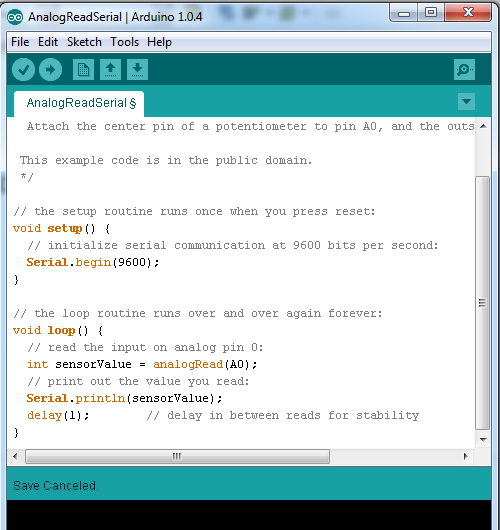
\includegraphics[width=0.75\textwidth]{../Images/IDE.png}
	\end{figure}
}

\frame
{
	\frametitle{Integrated developement environment}
Users only need define two functions to make a runnable cyclic executive program:	
	\begin{itemize}
	\item setup(): a function run once at the start of a program that can initialize settings
    \item loop(): a function called repeatedly until the board powers off
	\end{itemize}
}

\frame
{
	\frametitle{The Sensors}
	\begin{itemize}
	\item Temperature Sensor TMP36
	\item LDR GL5528
	\end{itemize}
}

\frame
{
	\frametitle{Temperature Sensor TMP36}
	\begin{figure}[htbp]
	\begin{minipage}[t]{4.65cm}
	\vspace{1pt}
	\centering
	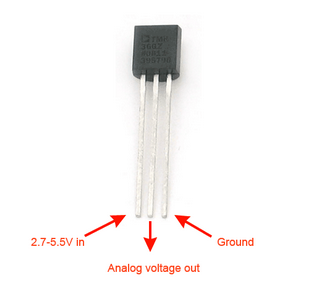
\includegraphics[width=\textwidth]{../Images/TMP36.png}
	\end{minipage}
	\hfill
	\begin{minipage}[t]{5cm}
	\vspace{10pt}
	\begin{enumerate}
	\item These sensors use a solid-state technique to determine the temperature. 
	\item They use the fact as temperature increases, the voltage across a diode increases at a known rate. 
	\item By precisely amplifying the voltage change, it is easy to generate an analog signal that is directly proportional to temperature. 
	\end{enumerate}
	\end{minipage}
	\end{figure}
	
}

\frame
{
	\frametitle{LDR GL5528}
	\begin{figure}[htbp]
	\begin{minipage}[t]{4.5cm}
	\vspace{0pt}
	\centering
	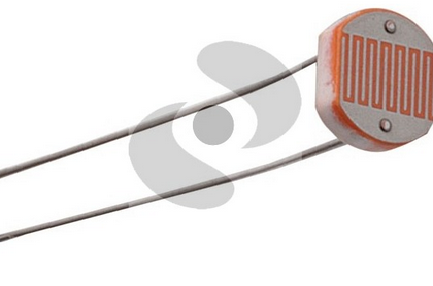
\includegraphics[width=\textwidth]{../Images/GL5528.png}
	\end{minipage}
	\hfill
	\begin{minipage}[t]{5cm}
	\vspace{10pt}
	\begin{itemize}
	\item GL5528 Photo Resistor (Light Depend Resistor). Photoresistor is a resistor which made of semi-conductor material,and the conductance changes with luminance variation.
	\item Applications:Photometry, Photoelectric Control, Light control lamp, Light control switch, Electronic Toy
	\end{itemize}
	\end{minipage}
	\end{figure}
	
}


%%%%%%%%%%%%%%%%%%%%%%%%%%%%%%% Estimation %%%%%%%%%%%%%%%%%%%%%%%%%%%%%%%%%%%%%%%%%%%%%
\section{Function Point Analysis}
\frame
{
	\frametitle{Function Points}
	\begin{enumerate}
	\item Defining the Unadjusted Function Point Count
	\item Determining the Value Adjustment Factor
	\item Determining Function Points
	\end{enumerate}
}

\subsection{Defining the Unadjusted Function Point Count}
\frame
{
	\frametitle{Defining the Unadjusted Function Point Count}
	\begin{figure}[h!]
  		\centering
    	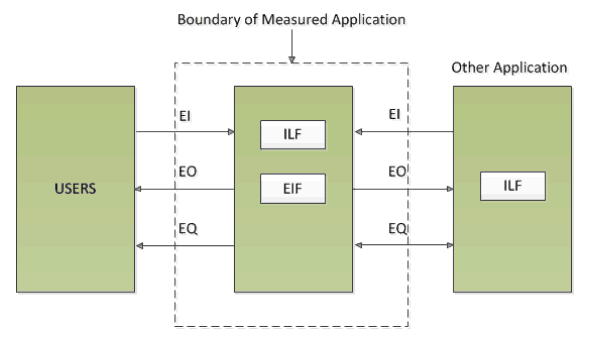
\includegraphics[width=0.85\textwidth]{../Images/FP_model.png}
		\caption{Boundary of MA}
	\end{figure}
}

\frame
{
	\frametitle{Unadjusted Function Point Count and Multipliers}
	\begin{figure}[h!]
  		\centering
    	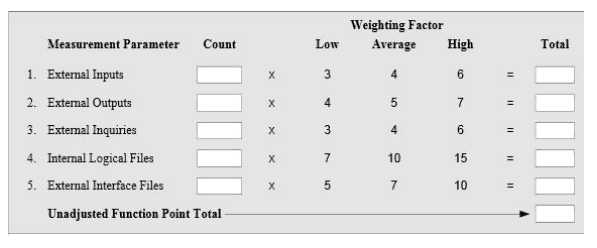
\includegraphics[width=\textwidth]{../Images/FP.png}
	\end{figure}
}

\subsection{Determinig the Value Adjustment Factor}
\frame
{
	\frametitle{Determinig the Value Adjustment Factor}	
	\begin{figure}[h!]
  		\centering
    	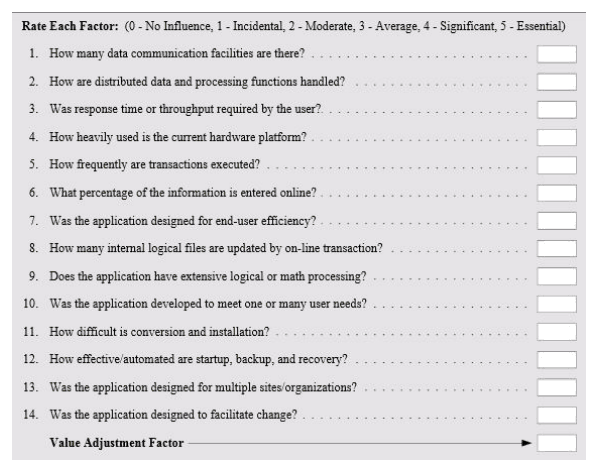
\includegraphics[width=0.85\textwidth]{../Images/FP_2.png}
		\caption{Total Degree of Influence}
	\end{figure}
}

\subsection{Determining Function Points}
\frame
{
	\frametitle{Determining Function Points}
	\begin{tabular}{|l|l|l|}
	\hline
	Project & Function Points 	& Man-Months 	\\ \hline
	ASD 	& 11 				& 1				\\ \hline
	KWO 	& 24 				& 2				\\ \hline
	RMD 	& 53 				& 5				\\ \hline
	WBO 	& 72 				& 6				\\ \hline
	\end{tabular}
}

\frame
{
	\frametitle{Determining Function Points}
	\begin{tabular}{|l|l|l|}
	\hline
	Project & Function Points 	& Man-Months 	\\ \hline
	ASD 	& 11 				& 1				\\ \hline
	Arduino	& 22				& 1.2			\\ \hline
	KWO 	& 24 				& 2				\\ \hline
	RMD 	& 53 				& 5				\\ \hline
	WBO 	& 72 				& 6				\\ \hline
	\end{tabular}
}

%%%%%%%%%%%%%%%%%%%%%%%%%%%%%%% System Architecture %%%%%%%%%%%%%%%%%%%%%%%%%%%%%%%%%%
\section{System Architecture}
\subsection{The Sensor}
\frame
{
	\frametitle{The Sensors}
	We are using two Sensors:	
	\begin{itemize}
	\item Temperature Sensor TMP36
	\item Light Dependant Resistor GL5528	
	\end{itemize}
}

\frame
{
	\frametitle{Temperature Sensor}
	\begin{figure}[h!]
  		\centering
    	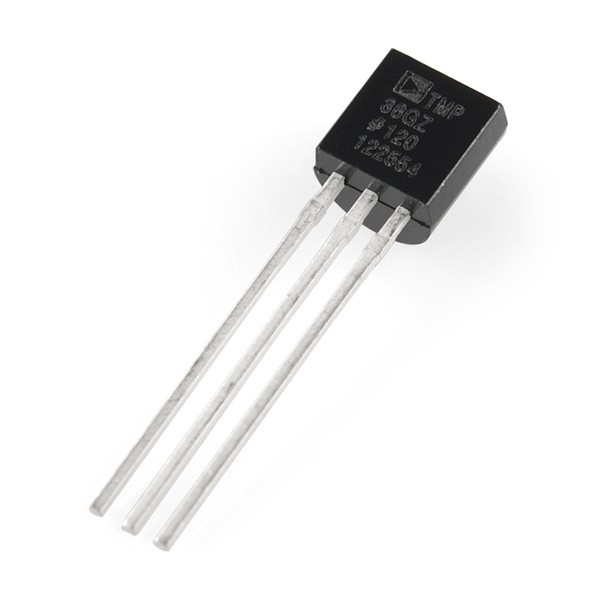
\includegraphics[width=0.5\textwidth]{../Images/Temp.jpg}
		\caption{TMP36}
	\end{figure}
}

\frame
{
	\frametitle{Temperature Sensor}
	Following Specification:
	\begin{itemize}
	\item outputs voltage depending on the temperature
	\item relation is linear
	\item Temperature Range: $-40^{\circ}$C to $125^{\circ}$C
	\item scalefactor of 10mV/$^{\circ}$C
	\item Accuracy of $\pm1^{\circ}$C at 25$^{\circ}$ and $\pm2\%$ in the range of $-40^{\circ}$C to 125$^{\circ}$C
	\end{itemize}
}

\frame
{
	\frametitle{Temperature Sensor}
	To calculate the Temperature in $^{\circ}$Celsius we use the formula:\\
	\begin{equation*}
	Temp = \frac{Voltage - 500}{10} 
	\end{equation*}
}

\frame
{
	\frametitle{Light Dependant Resistor}
		\begin{figure}[h!]
  		\centering
    	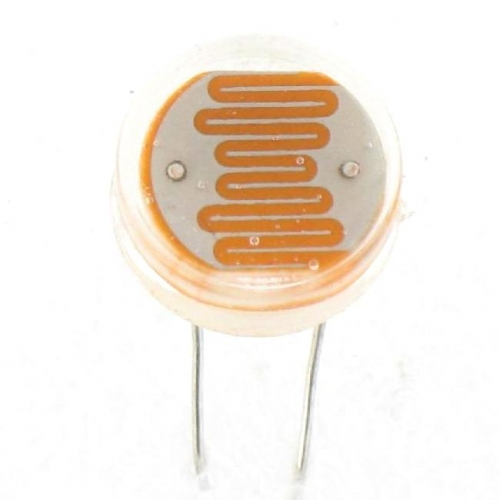
\includegraphics[width=0.5\textwidth]{../Images/Light.jpg}
		\caption{GL5528}
	\end{figure}
}

\frame
{
	\frametitle{Light Dependant Resistor}
	Following Specification:
	\begin{itemize}
	\item not precise enough to measure the light level
	\item only measure darkness from lightness
	\item Reliable perfomance
	\item linear relation
	\end{itemize}
}

\frame
{
	\frametitle{Light Dependant Resistor}
	To get the light value in Lux you have to do following steps:
	\begin{enumerate}
	\item Get Voltage of Resistor
	\item Get Resistor Value with formula:
	\begin{equation*}
		\frac{5.0 - Light Voltage}{lightv} * 10000
	\end{equation*}
	\item Get Lux with formula:
	\begin{equation*}
		10*\frac{14000}{Light Resistor}^\frac{1}{0.7}
	\end{equation*}
	\end{enumerate}
}

\frame
{
	\frametitle{Error Calculation}
	\begin{itemize}
	\item calculate quantisation error
	\item Temperature: $\pm$1 Degree
	\item Light: too high $\rightarrow$ only measure dark or bright of light
	\end{itemize}
}

\subsection{ZigBee Network}
\frame
{
	\frametitle{ZigBee Network}
	
	\begin{itemize}
	
	\item The Nodes in our WSN communicate in a ZigBee Network
	\item ZigBee Networks need a coordinator. The Collector will be the coordinator.
	\item The measuring Nodes will function either as End-Nodes or Routers
	\begin{itemize}
		\item{For the programming of the Nodes, this is irrelevant}
	\end{itemize}
	
	\end{itemize}
}

\frame
{
	\begin{itemize}
	
	\item As Radio Modules we are using XBee Modules from Digi
	\item They are attached to the Arduino's using Wireless Shields.
	\item To Adress the XBee Modules in the Software, we use the xbee-arduino Library
	\item The ZigBee adress of the coordinator will be hardcoded into the measuring Nodes Software
	\item The ZigBee Adress of the Measuring Nodes will be hard coded into the Coordinators Software
	\end{itemize}
}

\frame
{
	\frametitle{Communication}

	\begin{itemize}
	\item The coordinator will request Measurements from the Measuring Nodes
	\item The Message looks like this:
	\end{itemize}
	
	\begin{table}
    \begin{tabular}{|l|l|l|}
    \hline
    Byte(s) & content  & meaning                            \\ \hline
    1       & 'R'=0x52 & identifier for Measurement Request \\ \hline
    \end{tabular}
	\end{table}
}


\frame
{

	\begin{itemize}
	
	\item On Request, the Pond Measuring Node will Respond by this Message:
	
	\end{itemize}
	
	\begin{table}
    \begin{tabular}{|p{3cm}|p{3cm}|p{3cm}|}
    \hline
    Byte(s) & content  & meaning                                      \\ \hline
    1       & 'W'=0x57 & identifier for Measurement response          \\ \hline
    2-5     & float    & float for temperature measurement in Celsius \\ \hline
    6-9     & float    & float for light intensity in Lux             \\ \hline
    \end{tabular}
	\end{table}
}

\frame
{
	\begin{itemize}
	\item The Weather Measuring Node Responds with this Message:
	\end{itemize}
	
	\begin{table}[h]
    \begin{tabular}{|p{3cm}|p{3cm}|p{3cm}|}
    \hline
    Byte(s) & content  		& meaning                            \\ \hline
    1       & ''P'= 0x50 	& identifier for Pond measuremnt response \\ \hline
    2-5		& float			& float for temperature measurement in Celsius \\ \hline
    \end{tabular}
	\end{table}
}

\subsection{The Collecting Node}
\begin{frame}
	\frametitle{The Collecting Node}
	\begin{itemize}
		\item The Collecting Node takes the following Responsibilities:
		\begin{itemize}
			\item ZigBee Coordinator Role
			\item Know Daytime and Date by using NTP
			\item Request and receive Measurements
			\item Store all Data
			\item act as TCP Server, providing stored Data to Clients
		\end{itemize}
		\item The collector consists of:
		\begin{itemize}
			\item Arduino Ethernet
			\item Wireless Shield
			\item XBee Module
			\item micro SD-Card
		\end{itemize}
	\end{itemize}
\end{frame}




\begin{frame}
	\frametitle{Behavior}
	\begin{itemize}
		\item on startup, and every 24 hours, the collector will synchronize its stored daytime vie NTP
		\item every full and half hour, the collector will request a Measurement from the Measuring Nodes
		\item The Measuring Nodes have 30 Seconds to respond, otherwise their answer will be ignored
		\item After 30 seconds, or when both Measuring Nodes answered, the measurements get stored
	\end{itemize}
\end{frame}



\begin{frame}
	\frametitle{Software Architecture}
	\begin{itemize}
		\item Since the Collecting Node takes several responsibilities, it is necessary to partition the Software into components
		\item This components group specific kinds of functionalities.
		\item Those components are realised by implementing so called Arduno Libraries
		\begin{itemize}
			\item The Arduini Plattform allows the developer to write his own Libraries.
			\item A Library consists of a class, that can be instantiated in the main sketch
			\item Arduino Libraries are a way of using OOP-Techniques in the otherwise simplified Arduino Programming Language
		\end{itemize}
	\end{itemize}
\end{frame}



\begin{frame}
	\frametitle{Software Components}
			\begin{figure}[h!]
  		\centering
    	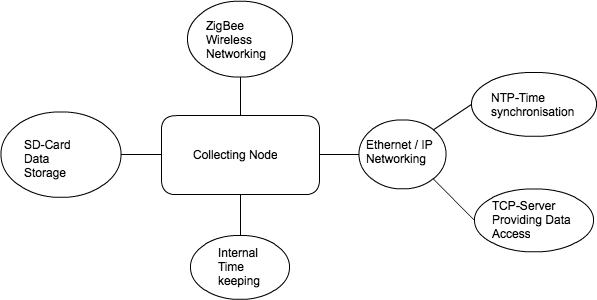
\includegraphics[width=\textwidth]{../Images/collector_software_components.png}
		\caption{Collector: Software Components}
	\end{figure}
\end{frame}

\begin{frame}
	\frametitle{Data Storage}
	\begin{itemize}
		\item The collector stores all data in a file on its SD Card
		\item The File is a CSV-File (Coma separated Values) with the following Format:
		\item \textbf{hh,mm,ss,dd,mm,yyyy,pppp,aaaa,llll}
		\item each Line in this file represents a complete measurement of the System at a certain point in time
		\item New Measurements add lines to the file
	\end{itemize}
\end{frame}

\begin{frame}
	\frametitle{Data Storage}
	\begin{itemize}
		\item A missing Value might be left out (But all comas stay to preserve the format)
		\item Example: \textbf{00,30,15,13,05,2013,11.5,9.7,}
		\item Means: At 00:30:15 on the 13th of May 2013, the Pond Temperature was 11.5C, the Air Temperature was 9.7C, and the light level was unknown
	\end{itemize}
\end{frame}


\subsection{The Measuring Nodes}

\frame
{
	\frametitle{The Measuring Nodes}
	\begin{itemize}
	\item Measurement Kit $\rightarrow$ Arduino Uno + Wireless Shield + XBee Module + 	Sensor Module	
	\item Sensor Module is different for Pond and Weather Measurement Station
	\item act as an ZigBee EndNode
	\item check if Coordinator has sent request
	\item if true send response to Coordinator	
	\end{itemize}
}

\frame
{
	\frametitle{The Measuring Nodes}
	\begin{figure}[h!]
  		\centering
    	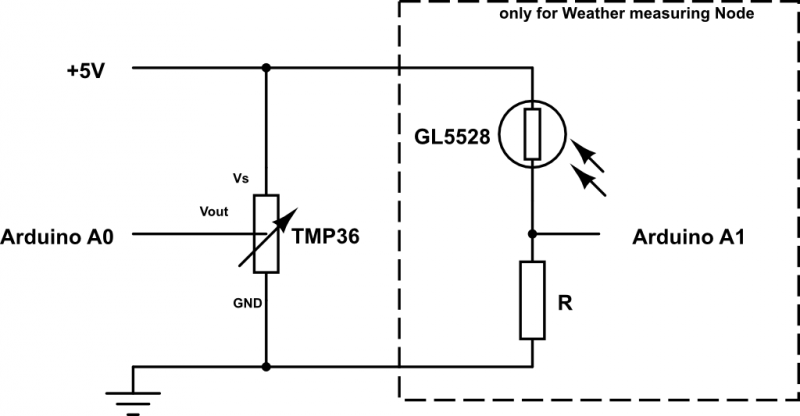
\includegraphics[width=\textwidth]{../Images/Circuit.png}
		\caption{Measuring Node Circuit}
	\end{figure}
} 

\frame
{
	\frametitle{Weather Node}
	\begin{itemize}
	\item outside node 
	\item measure Temperature and Light Intensity
	\item Send data via payload in a tx packet to Collector Node
	\end{itemize}		
}

\frame
{
	\frametitle{Pond Node}
	\begin{itemize}
	\item inside node
	\item measure Temperature in a pond
	\item Send data via payload in a tx packet to Collector Node
	\end{itemize}
	
}

\subsection{Application}
\frame
{
	\frametitle{Application}
	
	\begin{itemize}
	
	\item The application is used to access the collected data from the WSN
	
	\item The Data is displayed in a Textarea and Graphs
	
	\item The Data can then be exportet as the same CSV File as stored on the collector
	
	\item The exportet File can then be used in other applications like GNUPlot or SciLab.
	
	\end{itemize}

}


%%%%%%%%%%%%%%%%%%%%%%%%%%%%%%%%%%%% Project Results %%%%%%%%%%%%%%%%%%%%%%%%%%%%%%%%%%
\section{Project Results}
\frame
{
	\frametitle{Collecting Node}
	\begin{itemize}
	\item The Collecting Node has the most complex architecture
	\item unfortuantly the Collecting Node could not be finished on time
	\begin{itemize}
	\item some of the Collecting Nodes Software Components are finished (SD-Card Handling, Time and Date Awareness)
	\item but other Components could not be implemented
	\item The problem with implementing those Components is related to the Arduino Developement Environment
	\end{itemize}
	\end{itemize}
}

\frame
{
	\frametitle{Problems with the Arduino IDE}
	\begin{itemize}
	\item The Arduino Language \& IDE are made to be simple and easy to learn for Beginners
	\item But those simplifications also enforce limitations for the developer
	\begin{itemize}
	\item Writing Libraries by using other libraries is problematic $\rightarrow$ IDE does not link in the necessary object files
	\item there is no way of debugging Arduino sketches
	\end{itemize}
	\end{itemize}
}

\frame
{
	\frametitle{Problems with the Arduino IDE}
	\begin{itemize}
	\item Professionell IDEs for Microcontrollers provide possibilities to debug code that is running on the hardware
	\item This allows access to the processors for example registers or memory 
	\item It is possible to comprehend what is going wrong
	\item Without Debugging, the possibilities to understand not working code are very limited
	\item It took too much time, so the Collecting Node could not be finished on time
	\end{itemize}
}

\frame
{
	\begin{center}
	Demonstration
	\end{center}

}



%%%%%%%%%%%%%%%%%%%%%%%%%%%%%%% End %%%%%%%%%%%%%%%%%%%%%%%%%%%%%%%%%%%%%%%%%%%%%%%%%%%%
\frame
{
	\begin{center}
	Thank you for your attention!
	\end{center}
}

\end{document}
       
 